\documentclass[10pt,twocolumn,letterpaper]{article}

\usepackage{cvpr}
\usepackage{times}
\usepackage{epsfig}
\usepackage{graphicx}
\usepackage{amsmath}
\usepackage{amssymb}
\usepackage{enumitem,amsthm,amsfonts,subfig,float,multirow}
\usepackage[font=small,labelfont=bf]{caption}
\usepackage[none]{hyphenat}
\graphicspath{{figures/v1/}}
%-----------------------
% TIKZ
% -----------------------
\usepackage{tikz}
\usetikzlibrary{arrows,positioning}
\tikzstyle{state}=[draw, fill=white, align=center]
\tikzstyle{sum}=[draw, circle, fill=white, align=center, inner sep=1,outer sep=0]
\usepackage[breaklinks=true,bookmarks=false]{hyperref}


%------------------------
% CVPR
% -----------------------


\cvprfinalcopy % *** Uncomment this line for the final submission
%\def\cvprPaperID{****} % *** Enter the CVPR Paper ID here
\def\httilde{\mbox{\tt\raisebox{-.5ex}{\symbol{126}}}}
% Pages are numbered in submission mode, and unnumbered in camera-ready
%\ifcvprfinal\pagestyle{empty}\fi
\setcounter{page}{1}



%------------------------
% MATH
% -----------------------
   \newcommand{\p}{\mathbb{P}}
   \newcommand{\e}{\mathbb{E}}
   \newcommand{\R}{\mathbb{R}}
   \newcommand{\X}{\mathcal{X}}
   \newcommand{\LL}{\mathcal{L}}
   \newcommand{\Q}{\mathbf{Q}}
   \newcommand{\W}{\mathbf{W}}
   \newcommand{\indep}{\mathrel{\perp\mspace{-10mu}\perp}}
   \newcommand{\nindep}{\centernot{\indep}}
   \renewcommand\theequation{E\arabic{equation}}


\begin{document}

%%%%%%%%% TITLE
\title{Object recognition \& Computer vision\\
Project report - MVA 2015/2016\\
\textit{Training Convolutional Networks with Noisy Labels}}

\author{Maha ELBAYAD\\
ENS Cachan\\
\href{mailto:maha.elbayad@student.ecp.fr}{\tt maha.elbayad@student.ecp.fr}}
\maketitle
%\thispagestyle{empty}

%--------------------------- ABSTRACT
\begin{abstract}
The performance of Convolutional neural networks depends on the amount of labeled samples and their presumable quality, and since hand labelling is impractical, a shift toward semi-automatic labelling is inevitable which means more inaccuarte, subjective and sometimes misleading data that must be handled differently. For these reasons the method proposed in ~\cite{FB} handles the labels noise in an intuitive yet performant manner. 
\end{abstract}

\section{Introduction:}
The main objective of the studied paper is to assess the impact of the noise level on the classification error. The method outline consists of two phases: (1) training a convolutional neural network on the noisy data, (2) finetune the network with an additional constrained linear layer that would mimic a confusion matrix to retrieve a prediction closer to the true labels. Although the article deals with two types of noise, namely the \textbf{the label flip} and \textbf{the outlier}, we would focus for this project solely on the label flip. 

\section{The method:}
\subsection{Noise modelling:}
Given a trining set $\X=\{x_n,y_n\}_{1\leq n\leq N}$ where $y_n$ is the true label of the entry $x_n$. $y_n\in\{1...K\}$ in the contest of a K-multiclass classification. The additional noise layer has optimally for weights the confusion matrix $\Q$ defined as:
\[\Q=(q_{ij})_{1\leq i,j\leq K},\:\forall i,j\in\{1,..K\}\:q_{ij}=\p(\tilde y=i|y=j)\]
Where $\tilde y$ is the noisy label. In other words $q_{ij}$ is the probability of the class $j$ being mistaken for class $i$

By the sum rule we can evaluate the noisy label as:
\begin{equation}
\p(\tilde y=i|x)=\sum_jq_{ij}\p(y=j|x)
\end{equation}

\subsection{The network architecture}
For the base network, prior to learning the confusion matrix, we implement the architecture proposed in~\cite{krizhevsky2012imagenet} with response normalization and pooling: the CNN contains 3 convolution layers and a single fully-connected layer whose output for the sample $x_n$, $(\mathit{fc}_{n,k})_{1\leq k\leq K}$ is fed to a softmax loss:
\begin{equation}
\LL(\W)=-\frac{1}{N}\sum_{i=1}^N\log(\hat p_{n,\tilde y_n}),\phantom{abc}\hat p_{n,k}=\frac{\exp(\mathit{fc}_{nk})}{\sum_k\exp(\mathit{fc}_{nk})}
\end{equation}
We denote with $\W$ the weights of this base network wich in addition to the matrix $\Q$ form the parameters of our model.
\begin{figure}[H]
  \centering
  \subfloat[Phase 1]{
    \centering
    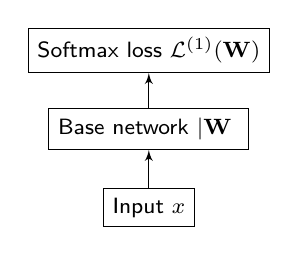
\begin{tikzpicture}[node distance=2.5cm,auto,>=latex',font=\sffamily\footnotesize]
        \node [state] (a) {Input $x$};
        \node [state] (b) [above of=a,node distance=1cm] {Base network $| \W$ };
        \node [state] (c) [above of=b,node distance=1cm] {Softmax loss $\LL^{(1)}(\W)$};
        \path[->] 
        (a) edge node {} (b)
        (b) edge node {} (c);
    \end{tikzpicture}
    } 
\subfloat[Phase 2]{
    \centering
    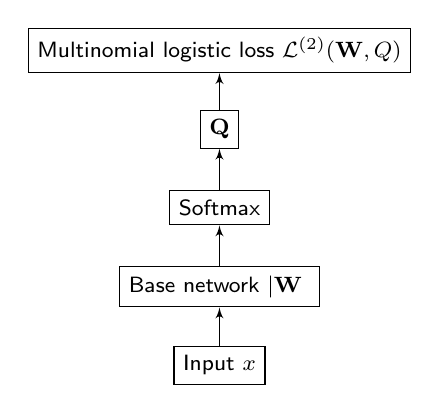
\begin{tikzpicture}[node distance=2.5cm,auto,>=latex',font=\sffamily\footnotesize]
        \node [state] (a) {Input $x$};
        \node [state] (b) [above of=a,node distance=1cm] {Base network $| \W$ };
        \node [state] (c) [above of=b,node distance=1cm] {Softmax};
        \node [state] (d) [above of=c,node distance=1cm] {$\Q$};
        \node [state] (e) [above of=d,node distance=1cm] {Multinomial logistic loss $\LL^{(2)}(\W,Q)$};
        \path[->] 
        (a) edge node {} (b)
        (b) edge node {} (c)
        (c) edge node {} (d)
        (d) edge node {} (e);
    \end{tikzpicture}
    }
    \caption{Model outline\label{outline}}
\end{figure}
\begin{figure}[H]
    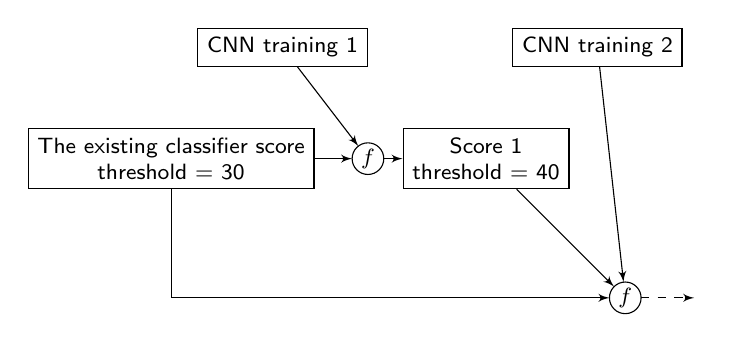
\begin{tikzpicture}[node distance=2.5cm,auto,>=latex',font=\sffamily\footnotesize,align=center]
        \node [state] (a) {The existing classifier score\\ threshold = 30};
        \node [state] (aa)[above right of =a, node distance=2cm] {CNN training 1};
        \node [sum] (suma)[right of =a, node distance=2.5cm] {$f$};
        \node [state] (b) [right of=suma,node distance=1.5cm] {Score 1\\threshold = 40};
        \node [state] (bb)[above right of =b, node distance=2cm] {CNN training 2};  
        \node [sum] (sumb)[below right of =b, node distance=2.5cm] {$f$};      
        \node  (c) [right of=sumb,node distance=1cm] {};
        \path[->] 
        (a) edge node {} (suma)
        (aa) edge node {} (suma)
        (suma) edge node {} (b)
        (b) edge node {} (sumb)
        (bb) edge node {} (sumb);
        \draw[->](a) |- node{} (sumb);
        \draw[dashed,->] (sumb) -- (c);
        
    \end{tikzpicture}
\end{figure}
Figure (\ref{outline}) illustrates the outline of the model where for the second phase we finetune the parameter $\W$ in addition to the extra linear layer with weights $\Q$. As $\Q$ expects probabilities for its input we insert a softmax layer to process the fully-connected layer's output. For similar reasons we use the multinomial logistic loss as the outputs are already a probability distribution.
\begin{equation}
\LL^{(2)}(\W,Q)=-\frac{1}{N}\sum_n\log \hat p(\tilde y=y_n|x_n,\W,\Q)
\label{eq3}
\end{equation}

\subsection{The confusion layer}
The article proves that minimizing the loss of (\ref{eq3}) with an additional regularizer forces the predicted distribution $\Q^*$ from the combined model to be as close as possible to the true confusion matrix $\Q$. To do so we use a weight decay on $\Q$ which will diffuse it.\\

In addition to the weight decay, and as we want $\Q$ to be optimally a stochastic matrix along its second dimension (each column sums to 1) we will scale the matrix $\Q$ at each each forward propagation.

\section{Experiments}
\section{The environment}
For our experiments we use Caffe, the deep learning framework by the BVLC~\cite{jia2014caffe}, to implement our confusion layer which is a tweaked version of the \texttt{innerProduct} layer. The training of the baseline networks has been performed on a GPU node of the Mesocentre de calcul de Centrale Paris, while the finetuning is done on CPU.

\subsection{CIFAR10}
We compare the performance of the model with and without the confusion layer on a manually corrupted dataset at variant noise levels. We're using CIFAR10~\cite{krizhevsky2009learning} a subset of 80 million Tiny Images dataset of natural images labeled into 10 object categories, 50k images are allocated to the training set and another 10k for the test set.

We train the first part of the model in 70000 iterations each with a batch of 100 images (i.e 140 epochs) with a learning rate varying as shown in table (\ref{lr})
\begin{table}[H]
\centering
\begin{tabular}{|c|c|c|c|}
\hline
Model&Epochs&lr&weight decay\\
\hline
\multirow{3}{*}{Baseline}& 1-120&1e-3& 1 on fc\\
&121-130&1e-4&..\\
&131-140&1e-5&..\\
\hline
\hline
Confusion&140-145&1e-4&.05 on Q\\
\hline
\end{tabular}
\caption{Learning rate policy\label{lr}}
\end{table}
While training the network, we keep track of the accuracy of the baseline network and the accuracy of the noise model prior to applying the confusion layer as it's supposed to absorb the noise and force the fully connected layer to output adapted scores. 
\begin{figure}
    \centering
    \includegraphics[width=8cm]{training}
    \caption{Accuracy during training at variant noise levels (CIFAR10)}
\end{figure}
We note that the reduction of the learning rate by a factor of 10 twice allows the network to further minimize the loss and boost its accuracy. The second jump of accuracy, albeit less noticeable, at the beginning of Q's finetuning proves that the layer is absorbing the noise as intended.
\begin{figure}
    \centering
    \includegraphics[width=7.5cm]{QQ}
    \caption{Confusion matrices: the learnt and the truly used to generate the noisy labels - the bright colors correspond to a value close to 1 - the diff value is for the $N_2$ distance between the two matrices (CIFAR10)\label{qq}}
\end{figure}


The figure (\ref{qq}) shows the difference between ground truth confusion matrix $\Q$ and the learnt $\Q^*$. Empirically this method has more impact at high noise level although the accuracy overall drops, but compared to the baseline model we get around +2 points of accuracy.
\begin{figure}
    \centering
    \includegraphics[width=8cm]{acc}
    \caption{Test accuracy when trained on 50k images with variant noise level (CIFAR10)}
\end{figure}
\subsection{Casia WebFace Database}
To test the method on realistic label noise we'll use a semi-automatically labeled subset of the Casia Webface database~\cite{yi2014learning} to perform a binary classification of facial images ($96\times 96$) with (1) or without (0) glasses.

If the model described above doesn't assume symmetric label noise (noise independent of the true label) it still does assume that the noise is independent of the input $x$. And with a minimal number of classes (binary classification) the number of additional parameters in Q is at its minimum. In these settings we will test the performance of the noise layer. 
In addition to that, having an unbalanced dataset with only 5\% of the images in the positive class (1) we will introduce an adapted noise with asymmetric level as well: a noise level referred to as $\alpha(1)$ corresponds to a flip from 0 to 1 with probability $\alpha$ and a flip from 1 to 0 with probability $19\times\alpha$ to maintain the distribution of the labels (5\% of class 1) and  $\alpha(2)$ corresponds to a flip from 0 to 1 with probability $\alpha$ and a flip from 1 to 0 with probability $\frac{\alpha}{10}$.
\begin{figure}
    \centering
    \includegraphics[width=8cm]{trainingM}
    \caption{Accuracy during training at variant noise levels (CASIA)}
\end{figure}

Our data is split into 4152 images for the training and 4661 for the test set.\\ The baseline network has 3 blocks of $\{$Conv, Pool, ReLU$\}$ and 2 fully-connected layers that lead to a softmax layer. The learning rate is decreasing throughout the 10000 training iterations ($\approx 154$ epochs):
\[\mathit{lr}(\mathit{iter})= \frac{0.01}{(1+iter\times 10^{-4} )^{0.75}},\:iter\leq 10^4\]
The $\Q$ matrix tuning takes 2500 iterations ($\approx 38$ epochs) with a fixed learning rate of $10^{-5}$ and a weight decay of $0.05$.

The learnt confusion matrix gets close to the true matrix on its second column - class 1, while often converging to $(1,0)^T$ in its first column - class 0 given the skewed distribution of the labels. Thus, the accuracy is weakly affected by the introduction of the layer.

\begin{table}[H]
\centering
\subfloat[Noise level 0.01(1)]{
\begin{tabular}{|cc||cc|}
\multicolumn{2}{c}{Learnt Q}&\multicolumn{2}{c}{True Q}\\
\hline
1.00 & 0.20 & 0.99 & 0.19\\
0.00 & 0.80 & 0.01 & 0.81\\
\hline
\end{tabular}}
\subfloat[Noise level 0.02(1)]{
\begin{tabular}{|cc||cc|}
\multicolumn{2}{c}{Learnt Q}&\multicolumn{2}{c}{True Q}\\
\hline
1.00 & 0.21 & 0.98 & 0.38\\
0.00 & 0.79 & 0.02 & 0.62\\
\hline
\end{tabular}}
\\
\subfloat[Noise level 0.1(2)]{
\begin{tabular}{|cc||cc|}
\multicolumn{2}{c}{Learnt Q}&\multicolumn{2}{c}{True Q}\\
\hline
1.00 & 0.06 & 0.90 & 0.01\\
0.00 & 0.94 & 0.10 & 0.99\\
\hline
\end{tabular}}
\subfloat[Noise level 0.2(2)]{
\begin{tabular}{|cc||cc|}
\multicolumn{2}{c}{Learnt Q}&\multicolumn{2}{c}{True Q}\\
\hline
1.00 & 0.00 & 0.80 & 0.02\\
0.00 & 1.00 & 0.20 & 0.98\\
\hline
\end{tabular}}
\caption{Confusion matrices: the learnt and the truly used to generate the noisy labels}
\end{table}

\section{Discussions}
Our implementation of the confusion layer in the way described in the article and with the columns normalization mentioned above does generally succeed to learn the confusion matrix, yet the layer in itself doesn't boost the performance of the network, especially in the case of natural noise. Nonetheless the learnt $\Q^*$ can be used to bootstrap the training set or simply for the small gain of accuracy given that the finetuning of $\Q$ doesn't require much computation.
%----------
% Biblio
%---------
{\small
\bibliographystyle{ieee}
\bibliography{egbib}
}
\end{document}
